\chapter{Gaussian Splatting for 360\degree spin stabilization}
\label{chapter:gausssplat}

\chapterwithfigures{\nameref*{chapter:gausssplat}} \chapterwithtables{\nameref*{chapter:gausssplat}}

\ifthenelse{\boolean{skipGauss}}{\endinput}{}


% Math symbol

\section{Introduction}
This final section extends the latest two sections that were mostly focused toward a research academic perspective. Core motivation rather lies here on the desire to apply \ac{NVS} latest advances on an industrial project, where processed images resolution are at least $10\times$ higher than ShapeNet-SRN \citep{chang2015shapenet,sitzmann2019scene} ones ($\sim$ 1-2K against $128\times128$). \ac{NeRF} have benefited over the latest few years from massive improvements against several directions; training time, camera pose requirements, inference speed, drastic model weight reduction \textit{etc}. 
However, \ac{NeRF}-based methods suffers from an intrinsic computational bottleneck at inference time. It requires to query the \ac{NeRF} roughly 500 millions times to generate a squared $2K\times2K$ image. As a direct consequence, one of the most acknowledged state-of-the-art method, termed Mip-NeRF360 \citep{barron2022mip}, is only able to render at < 0.1 \ac{FPS} a 1080p image. It would therefore be necessary to deploy a lot of \ac{GPU} resources and engineering refactorization to properly parallelize the source code in order to synthesize novel views at acceptable speed. 

We thus work in this section with a different set of constraints. First concerns the generalizable property we kept in the two previous sections. We do not aim anymore to build or rely on an algorithm that can synthesize a viewpoint from any image belonging to a specific class. We thus rather want to leverage on \textit{per-scene} framework, that would require a novel training as soon as we work with a new scenario. Furthermore and as mentioned earlier, images we are now working with are closer to what clients could sent to any \ac{AI} SaS company, both regarding resolution and content. Finally, camera poses are no longer available as ground truth since real-world images CarCutter by Meero has to deal with are unposed. They thus must be first estimated using \ac{SFM} techniques (subsection \ref{subsec:gs-sfm}).

Core idea is rather to leverage on the very latest advances in neural rendering, mostly on \ac{GS} ones. \ac{GS} offers an extremely well balanced trade-off between rendering quality and training/inference requirements. Contrary to \ac{NeRF}-based methods, that are therefore often too slow to render high-resolution images, \ac{GS} shows an outrageously 100 \ac{FPS} performance, withtout relying on any neural network architecture. However, the \ac{NVS} paradigm we were used to deal with until now has heavely changed: View synthesis is not anymore infered given a source image and a camera transformation. As soon as \ac{GS} reconstructs the whole 3D scene through a set of 3D coloured gaussians, render a novel view now at a specific viewpoint only require a camera pose information.


\section{Background}
In order to be as close as possible to what was investigated for CarCutter and to remain consistent accross the experiments and tested methods, a single scene made of 36 views is used in this section. Figure \ref{fig:gs-original_scene} depicts such scene. This background section establishes fundamental concepts and algorithms that turn such an unordered and unposed finite set of images into an explicit 3D scene that can be rendered from any viewpoint. 

\begin{figure}[htb!]
  \centering
  \begin{subfigure}[b]{0.45\linewidth}
    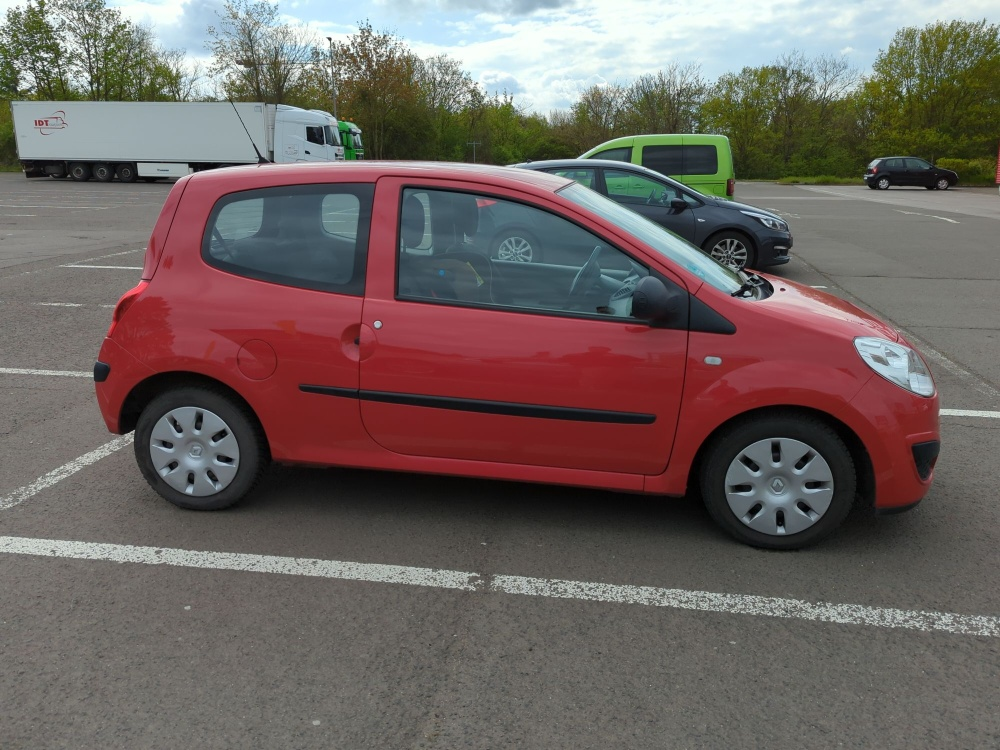
\includegraphics[width=\linewidth]{images/gaussiansplatting/gt/img-4.jpg}
    \caption{\textbf{A random view.} The view indexed \textit{0004} is represented here for an illlustrative purpose. }
    \label{fig:view-idx-4}
  \end{subfigure}
  \quad % Space between the figures
  \begin{subfigure}[b]{0.45\linewidth}
    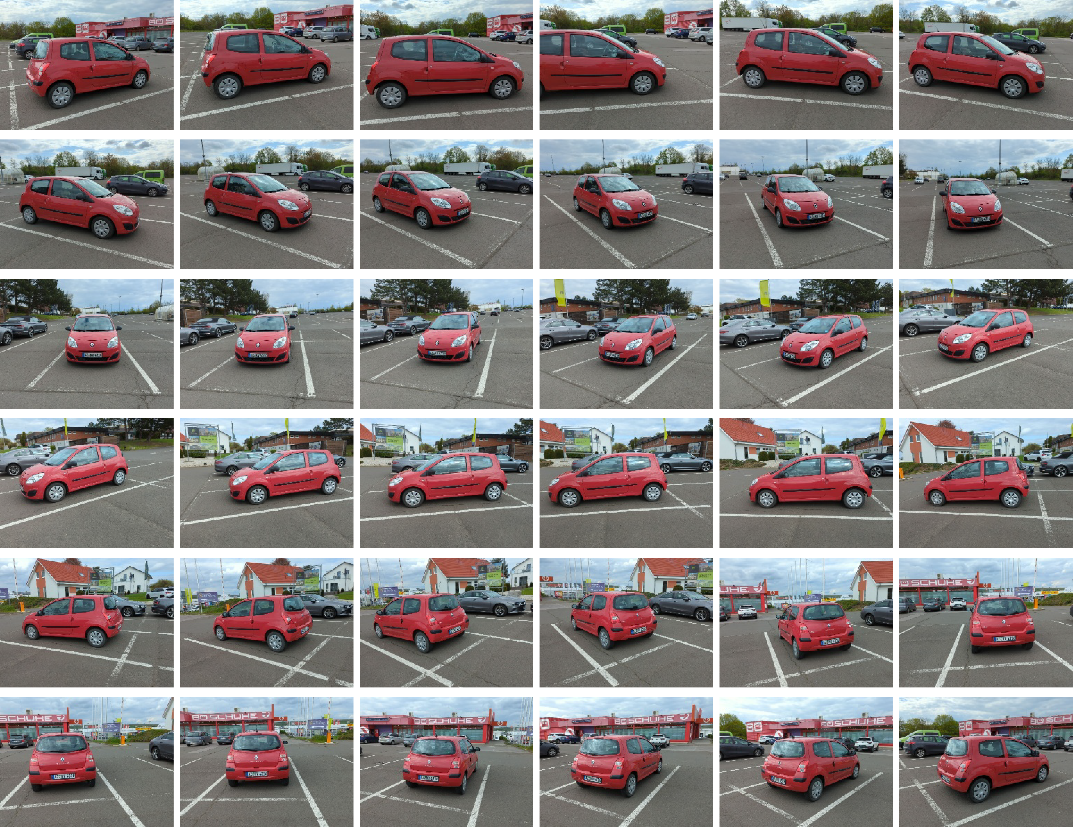
\includegraphics[width=\linewidth]{images/gaussiansplatting/original_scene.png}
    \caption{\textbf{Original scene.} Such a scene is typically what Carcutter is working with on a daily basis. A total of 36 unposed views has been acquired here. }
    \label{fig:gs-original_scene}
  \end{subfigure}
  \caption{\textbf{Scene set overview} The considered scene as 36 $1500\times2000$ photographs that were taken by hand without any tripod nor specific equipment. }
  \label{fig:gs-scene-dataset}
\end{figure}

\subsection{Camera pose estimation through SfM with COLMAP}
\label{subsec:gs-sfm}

\begin{figure*}[htb!]
    \center
  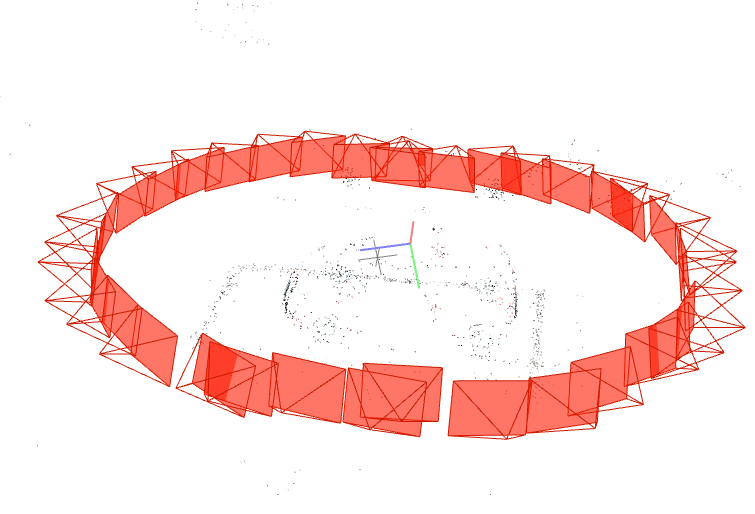
\includegraphics[height=8cm]{images/gaussiansplatting/colmap_sparsePC.png}
  \caption{\textbf{COLMAP 3D sparse reconstruction.} Given the set of unorded and unposed 36 views depicted below, COLMAP reconstructs an extremely sparse coloured point cloud with the corresponding estimated camera location. A total of $N=4105$ points has been registered here in this scenario.}
  \label{fig:gs-sfm}
\end{figure*}


\subsection{Gaussian Splatting}
\label{subsec:gs-gs}

It exists a plaethora of different ways to represent 3D data, either explicitly (such as point clouds, meshes) or implicitly. \ac{NeRF} implicitly embeds the whole structure and texture of a scene in its inner weights: an image is rendered by sampling points on casted rays and quering the architecture accordingly. \ac{GS} rather leverages on a 3D gaussian primitive to explicitly model the 3D scene and get a fully differentiable pipeline that can solely be supervised at 2D-image level. Figure \ref{fig:gs-overview} gives few insights regarding how such a pipeline is built.  


\begin{figure*}[htb!]
    \center
  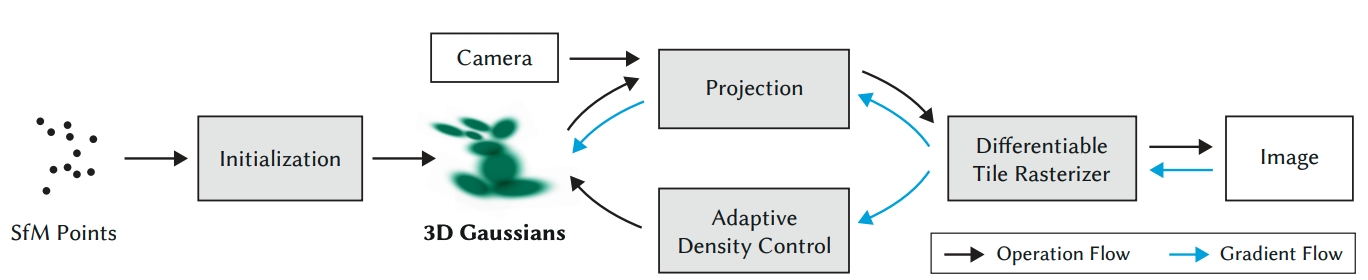
\includegraphics[width=\linewidth]{images/gaussiansplatting/overview-pipelineGS.png}
  \caption{\textbf{Gaussian Splatting pipeline overview.} Starting from a sparse 3D point cloud, \ac{GS} is designed on a lightweight and differentiable pipeline that does not involve any deep or shallow neural architectures.}
  \label{fig:gs-overview}
\end{figure*}


We present below the key steps that were defined in the original \ac{GS} seminal work \citep{kerbl20233d}.

\noindent \textbf{Initialization} From a sparse coloured \ac{SFM}-3D point cloud, refered as $\mathcal{P}\in\mathbb{R}^{N\times(3+3)}$, an associated set of 3D Gaussians $\mathcal{G}$ is build. Each primitive $g \in \mathcal{G}$ has therefore an attached set of attributes $\{\mu,\Sigma,c,\alpha\}$, defined by: 
\begin{itemize}
    \item A mean $\mu$, corresponding to the original point location in $M$. 
    \item A covariance $\Sigma$ $3\times3$ matrix, that must be positive semi-definite. Initialized to be isotropic. 
    \item A color $c$, represented using \ac{SH} coefficients. Additional information regarding \ac{SH} theory and construction can be found in the Appendix \ref{appendix:gs-sh}. 
    \item An opacity/transparency $\alpha$ value. 
\end{itemize}
These attributes that are going to be learned, for all gaussians in  $\mathcal{G}$ during training. While mean, color and opacity can be optimized without any constraints with gradient-descent based algorithm, $\Sigma$ has to remain semi-definite positive \footnote{\textit{i.e} $ \forall a \in \mathbb{R}^{3}: a^{T}\Sigma a \geq 0$} during training to represent a meaningful 3D coviance matrix. As holding this constraint during the optimization would be to complex, $\Sigma$ is factorized (as an eigendecomposition) in the world coordinate system via with a rotation $R$ (analytically expressed with 4 quaternions) and a scaling matrix $S$: 

\begin{equation}
    \Sigma = RSS^{T}R^{T}
\end{equation}
As any matrix expressed with $A^{T}A$ is always semi-definite positive, $\Sigma$ is now properly constrained. Term $RS$ has to be seen as scaled rotation matrix, where $R$ defines the Gaussian $g$ rotation in space and $S$ its size. 

Considering any point \textit{p} in the physical 3D space, a 3D gaussian $g$, has an influence over \textit{p} that can be expressed through: 

\begin{equation}
  f = \alpha\exp(-\frac{1}{2}(p-\mu)^{T}\Sigma^{-1}(p-\mu))
\end{equation}

\noindent \textbf{3D Gaussian projection} The 3D Gaussian parameters need to optimized during the training phase by only leveraging on an image-based supervision signal. The 3D ellipsoides must thus be render on 2D image plane in a differentiable manner and a corresponding 2D mean and covariance need to be derived from $\mu$ and $\Sigma$ for each gaussian using EWA splatting \citep{zwicker2001ewa}. 

Let's denote the world-to-camera extrinsic matrix W and the intrinsic K, the gaussian center is easily projected in 2D through the perspective projection: 

\begin{equation}
  \begin{bmatrix}
    u \\
    v \\
    z
  \end{bmatrix} = KW\mu
\end{equation}
and the 2D mean $\mu' = \begin{bmatrix}
  u/z \\
  v/z
\end{bmatrix}$ can be  thus expressed as:
\begin{equation}
  \mu' = K(W\mu/(W\mu_{z}))
\end{equation}
Regarding the 3D covariance, it can be expressed in 2D as:

\begin{equation}
  \Sigma'= JW\Sigma W^{T}J^{T}
\end{equation}

where $J = \partial \mu' / \partial \mu$ is the Jacobian of the mean projection formula. Additional information regarding this latest equation can be found in Appendix \ref{appendix:cov}. 

\noindent \textbf{Adaptative Density Control (ADC)} 
As the original \ac{SFM} point cloud can be extremely sparse, authors from \cite{kerbl20233d} implement both a densification and pruning strategy during training. The pruning is quite simple yet effective: any 3D gaussian that has an opacity $\alpha$ below a fixed threshold $\epsilon_{\alpha}$ during training is removed from $\mathcal{G}$. 

The densification stategy is not as immediate insofar as it required to both address under-reconstructed areas (where an insufficient number of gaussians are present) and over-reconstructed areas (where gaussians are too large) of the scene, as depicted on Figure \ref{fig:gs-densification}. 

\begin{figure*}[htb!]
  \center
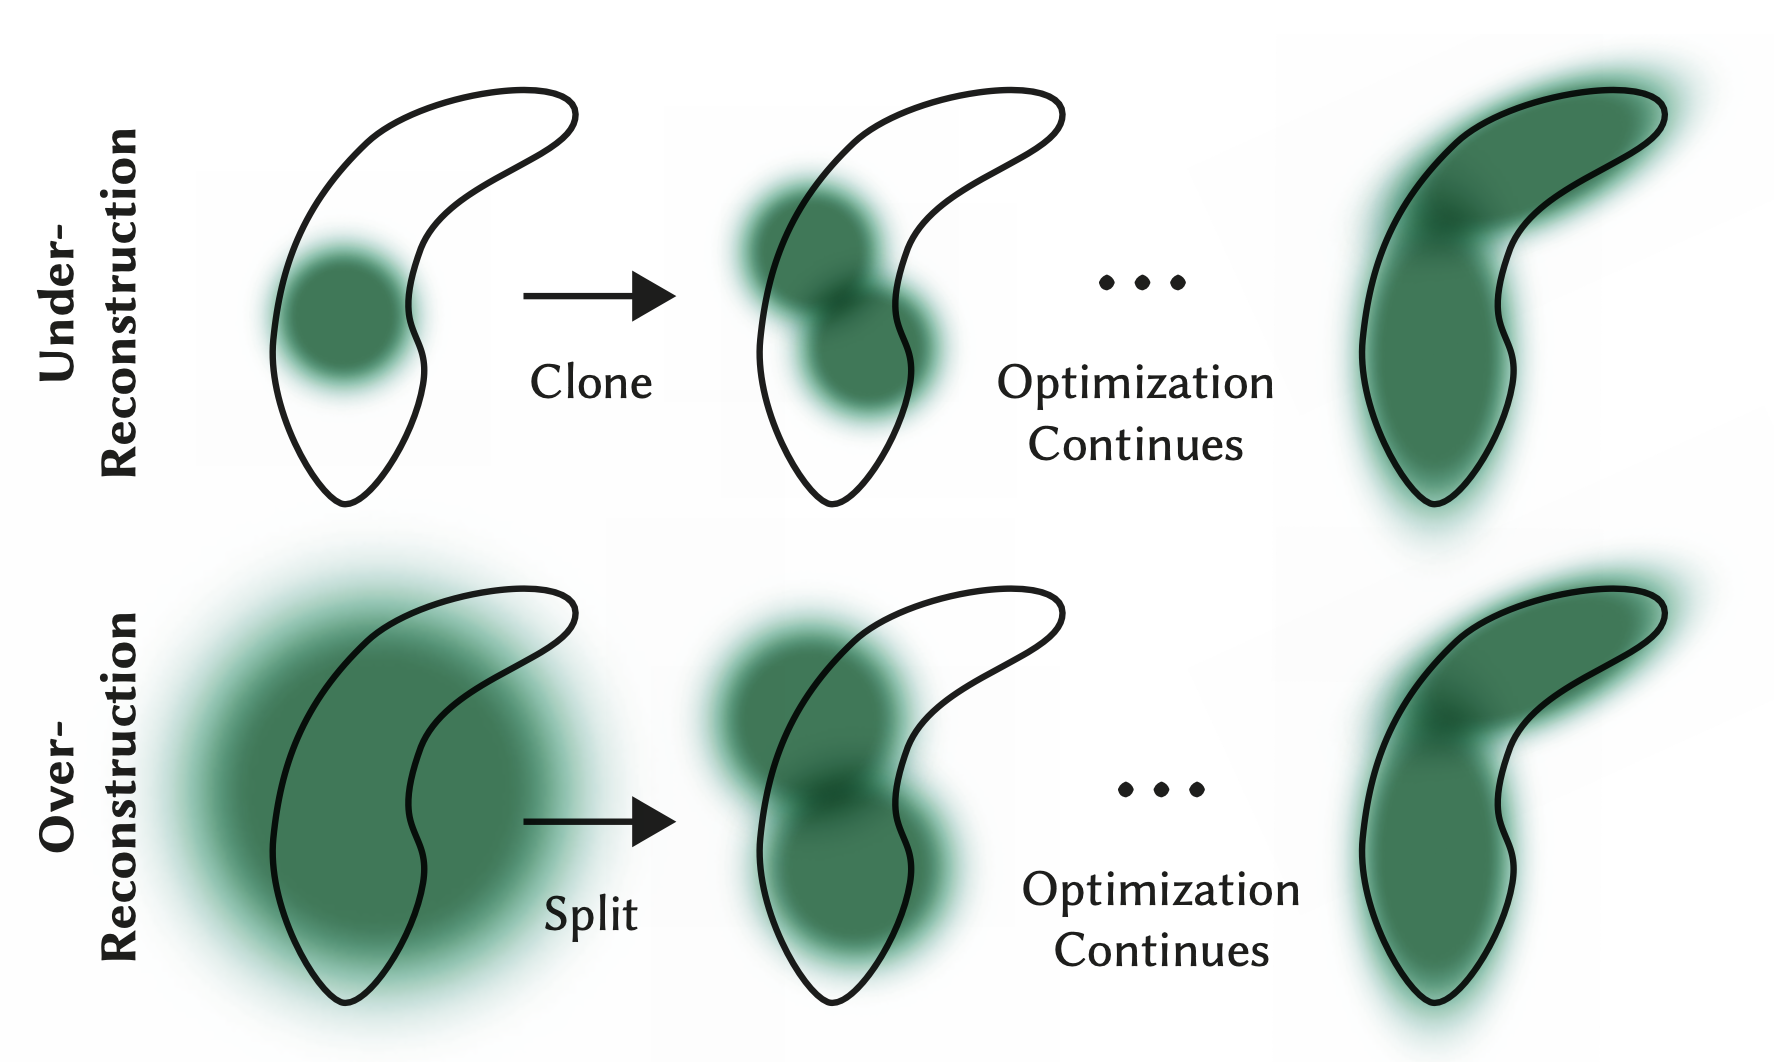
\includegraphics[width=.7\linewidth]{images/gaussiansplatting/densification-strategy.png}
\caption{\textbf{Densification Strategy.} By addressing both under and over-reconstructed areas, the densification strategy always increases the total number of gaussians but kept its associated total volume  constant in the \textit{split} stategy (contrary to the \textit{clone} one).}
\label{fig:gs-densification}
\end{figure*}

\section{Related Work}

\section{Method}
\subsection{Camera path stabilization}

As we should except, COLMAP camera poses that were estimated do not describe a lean and regular trajectory around the car (Figure \ref{fig:gs-camera-path-unstab}). We thus need to correct these poses in order to describe a circular camera path around the car. 


Merging the photographs from the scene depicted on Figure \ref{fig:gs-original_scene} leads to a too bumpy result from a camera path perpective. Transition between two views are unpleasant since images of the car are inconsistent from a distance and camera look at direction perspective: Figure \ref{fig:gs-unstabilized-gif} shows how a raw and uncorrected merge of these view into a \textit{.gif} animation looks like. 

\begin{center}
  \animategraphics[autoplay,loop, poster=0,width=\linewidth]{5}{images/gaussiansplatting/gt/img-}{0}{35}
  \label{fig:gs-unstabilized-gif}
  \captionof{figure}{\textbf{Unstabilized camera path} Resulting image merge into a \textit{.gif} animation is too erratic since corresponding camera path has not been stabilized.}
\end{center}

Let's denote $\mathcal{I}=\{I_{i}\}_{i=1}^{N}$ the set of N RGB images, paired with their associated viewpoint $\pi_{i}$, and  $\mathcal{C} = \{C^{(i)}\}_{i=1}^{N}$ the set of COLMAP-based camera centers. These centers are expressed in world coordinates as: 
\begin{equation}
  C^{(i)}=-R_{i}^{T}\times t_{i}
\end{equation}
 where $R_{i}$ and $t_{i}$ respectivelly account for the world to camera rotation and translation. The car centroid $O_{car}$ is directly built from the 3D tires location\footnote{which are also estimated by another algorithm that would not be described in this manuscript}: 

\begin{equation}
  \begin{split}
  O_{car} = t_{RL}^{(3D)} + & \frac{t_{1}+t_{2}}{2} -(t_{1}\otimes t_{2})\frac{\left\lVert t_{r}\right\lVert_{2}}{2} \\ \\
  & t_{1} = t_{FL}^{(3D)} - t_{RL}^{(3D)} \\
  & t_{2} = t_{RR}^{(3D)} - t_{RL}^{(3D)} 
  \end{split}
  \end{equation}

where $\otimes$ denotes the cross-product and $t_{FL}^{(3D)}$ the front-left 3D tire location.\footnote{The rear-right tires is thus denoted $t_{RR}^{(3D)}$} Considering the \ac{SVD} of $\mathcal{C}_{c} = \mathcal{C} - O_{car}$, the normal $\vec{n}$ of the 2D plane that fits the best $\mathcal{C}_{c}$ is expressed as the right singular vector whose singular value is the smallest. 

[Write down proper equation for 3D projection onto the plane / 2D coordinates on the plane, circle fitting and points projections on finally points projections onto this circle]

The camera path can thus stabilized at a fixed height around circle, as describe on Figure \ref{fig:gs-camera-path-stab}. We present in Appendix \ref{appendix:spherical-interp} how sperical interpolation can be used to evenly space these camera locations around the computed circle. 


\begin{figure}[htb!]
  \centering
  \begin{subfigure}[b]{0.45\linewidth}
    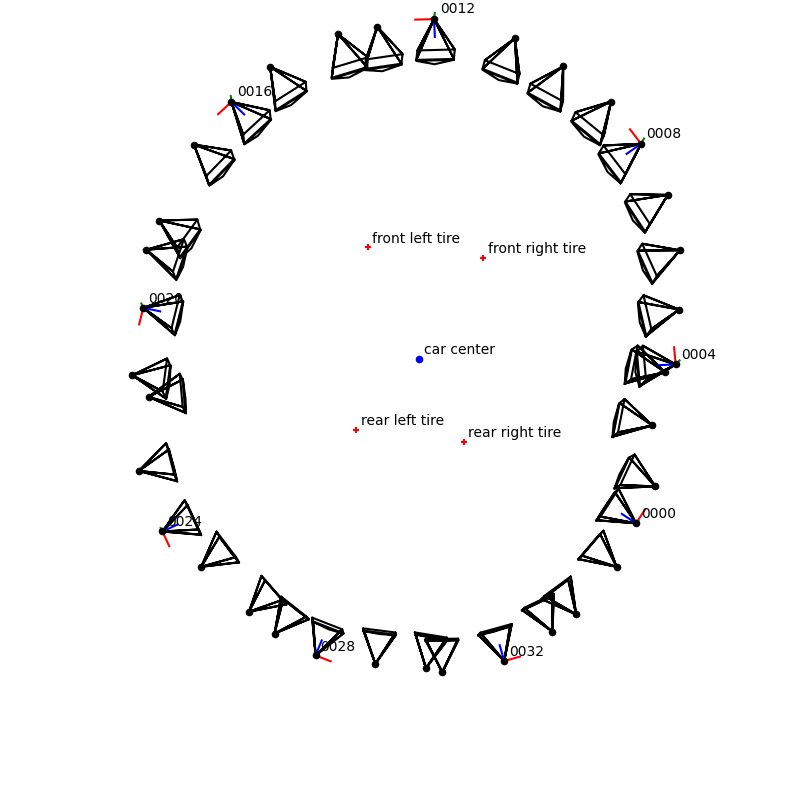
\includegraphics[width=\linewidth]{images/gaussiansplatting/camera-path-unstabilized.png}
    \caption{\textbf{Original camera path.} COLMAP predicted camera poses are unevenly spaced and do not describe a smooth path around the car. }
\label{fig:gs-camera-path-unstab}
  \end{subfigure}
  \quad % Space between the figures
  \begin{subfigure}[b]{0.45\linewidth}
    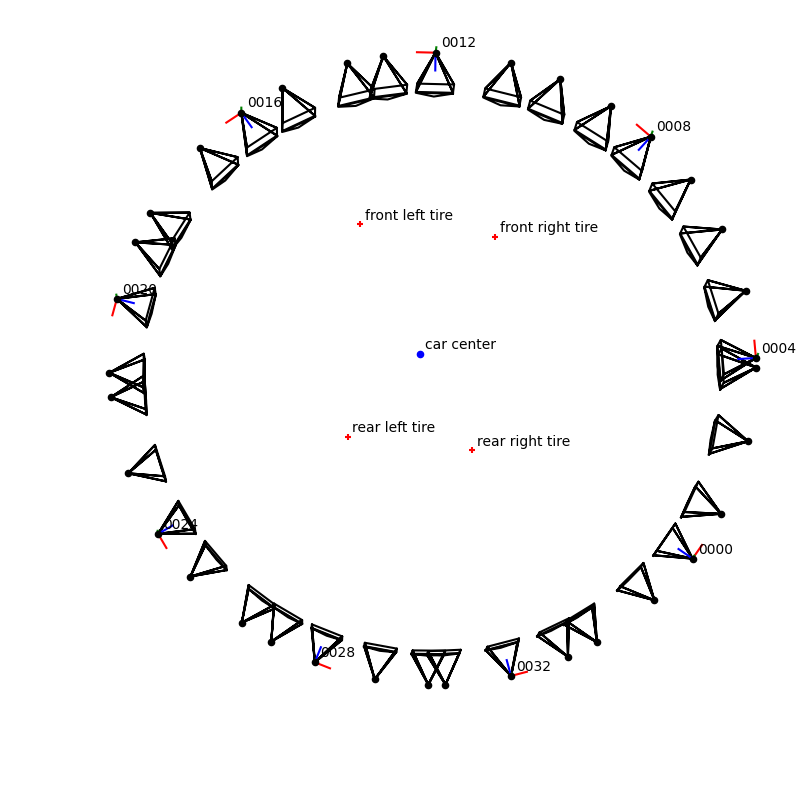
\includegraphics[width=\linewidth]{images/gaussiansplatting/camera-path-stabilized.png}
    \caption{\textbf{Corrected camera path.} Camera poses has been projected around a circle, centered around the computed car center.}
    \label{fig:gs-camera-path-stab}
  \end{subfigure}
  \caption{\textbf{Camera path set overview} Whereas camera centers have been set around a circle, they remain unevenly spaced.}
  \label{fig:gs-campath}
\end{figure}

\subsection{$360\degree$ with homography}

We present in this subsection the first and most straightforward way to obtained stabilized views from the scene: leveraging the perspective transformation theory. Indeed, such a transformation can be computed and applied to all the source views as soon as we get the orginal $\mathcal{C}$ and stabilized camera $\mathcal{C}_{stab}$ world locations. 

Given any camera center $C^{((i))}_{stab} \in \mathcal{C}_{stab}$, one can retrieve the corresponding rotation $R_{i}^{stab}$ in world coordinates through: 

\begin{equation}
  \begin{split}
    rot^{(i)}_{Z} & = - {\left[C^{((i))}_{stab}\right]}_{2}\\
    rot^{(i)}_{X} & = - e_{1} \otimes rot^{(i)}_{Z} \\
    rot^{(i)}_{Y} & = {\left[rot^{(i)}_{Z}\otimes rot^{(i)}_{X}\right]}_{2}
    \end{split}
\end{equation}
and 
\begin{equation}
R_{i}^{stab}  = \begin{bmatrix}
      rot^{(i)}_{X}\\
      rot^{(i)}_{Y} \\
      rot^{(i)}_{Z}
      \end{bmatrix}
\end{equation}

while the associated homography describing how $\pi_{i}$ moved from $C^{((i))}$ to $C^{((i))}_{stab}$ is trivially computed as: 

\begin{equation}
  \begin{split}
    H_{R}^{(i)} & = R_{i}^{stab}R_{i}^{T} \\
    H_{t}^{(i)} & = - R_{i}^{stab}(C^{((i))}_{stab} - C^{((i))})
  \end{split}
\end{equation}

The camera intrinsinc $K$ (that can also be estimated by COLMAP) enables, with $H^{(i)}$, to apply a perspective transformation on the corresponding view. We present on the Figure \ref{fig:gs-homography-view3} how the view index \textit{0003} has been transformed. 

\begin{figure}[htb!]
  \centering
  \begin{subfigure}[b]{0.45\linewidth}
    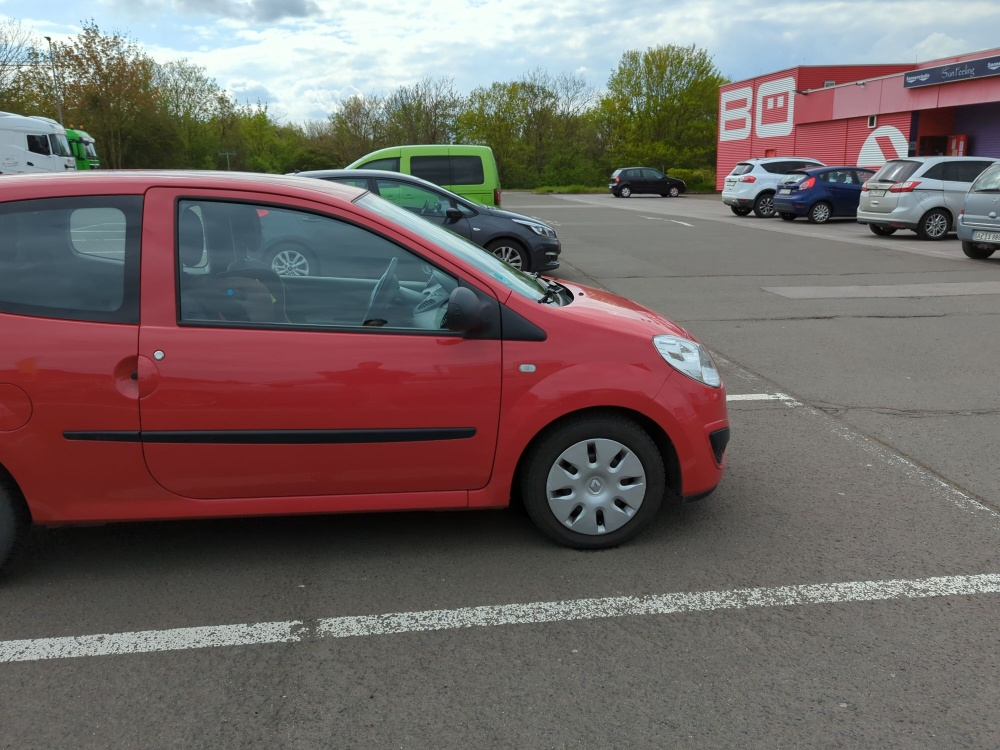
\includegraphics[width=\linewidth]{images/gaussiansplatting/gt/img-3.jpg}
    \caption{\textbf{Original view.}}
    \label{fig:view3}
  \end{subfigure}
  \quad % Space between the figures
  \begin{subfigure}[b]{0.45\linewidth}
    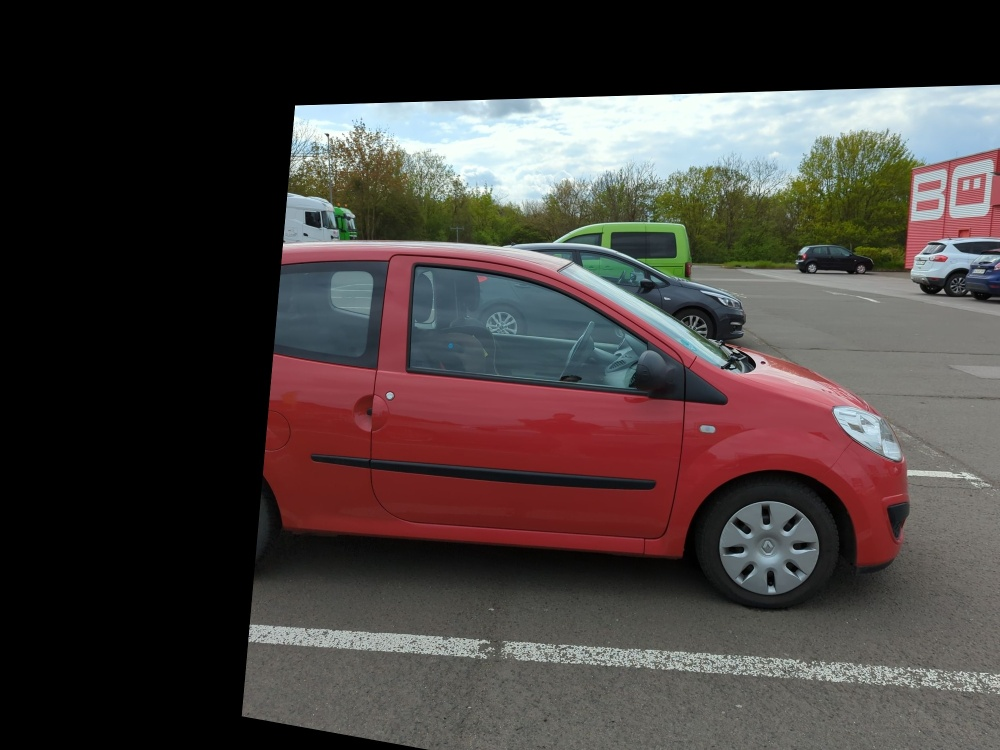
\includegraphics[width=\linewidth]{images/gaussiansplatting/stabhomo/img-3.jpg}
    \caption{\textbf{Perspective wrapped view.}}
    \label{fig:gs-view3-homo}
  \end{subfigure}
  \caption{\textbf{Perspective transformation based stabilization}. Whereas the car is now properly centered on the view, the car is cropped as the perspective transformation to apply was too drastic}
  \label{fig:gs-homography-view3}
\end{figure}

Once such transformation has been applied to the entire scene, the $360\degree$ spin tour is now properly stabilized and the corresponding animation cleaner than before, as shown on Figure \ref{fig:gs-stabilized-homo-gif}. 

\begin{center}
  \animategraphics[autoplay,loop, poster=0,width=\linewidth]{5}{images/gaussiansplatting/stabhomo/img-}{0}{35}
  \label{fig:gs-stabilized-homo-gif}
  \captionof{figure}{\textbf{Stabilized $360\degree$ spin path} The scene is now properly stabilized even though some perspective transformed views cropped the car.}
\end{center}

Car cropping is one the main limitation of this first solution and it cannot be triavially adressed. Besides, CarCutter clients often lack room to back up further when they shoot a car. There are therefore two causes that might lead to car cropping as any input view might also partially depict the car. Such a pure geometrical-based solution cannot fake or generate cars missing parts. 

\subsection{$360\degree$ with Gaussian Splatting}
\label{subsec:gs-vanilla_gs}
We investigate in this section the seminal work from \citep{kerbl20233d} on our scene. From a number of input views perspective, our scene might be considered as sparsed: research datasets used to train and test \ac{GS} often have hundreads of photographs. Since our scene is made of only 36 views, we used all of them to train the \ac{GS} model. 

We first present on the Figure \ref{fig:gs-view3} the rendering of the view indexed \textit{0003}, that was thus in the training set. As the entire 3D scene structure has been learned and is explicitly stored as a gaussian point cloud, one can render it at any locations and synthesize the whole car. 

\begin{figure}[htb!]
  \centering
  \begin{subfigure}[b]{0.45\linewidth}
    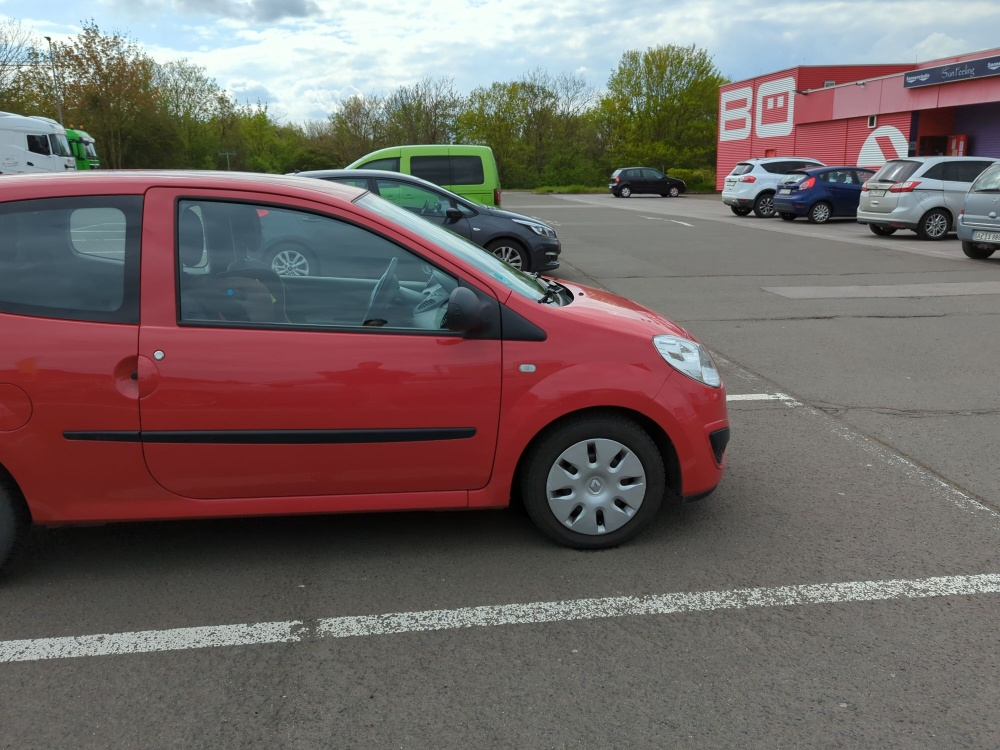
\includegraphics[width=\linewidth]{images/gaussiansplatting/gt/img-3.jpg}
    \caption{\textbf{Original view.}}
    \label{fig:view3}
  \end{subfigure}
  \quad % Space between the figures
  \begin{subfigure}[b]{0.45\linewidth}
    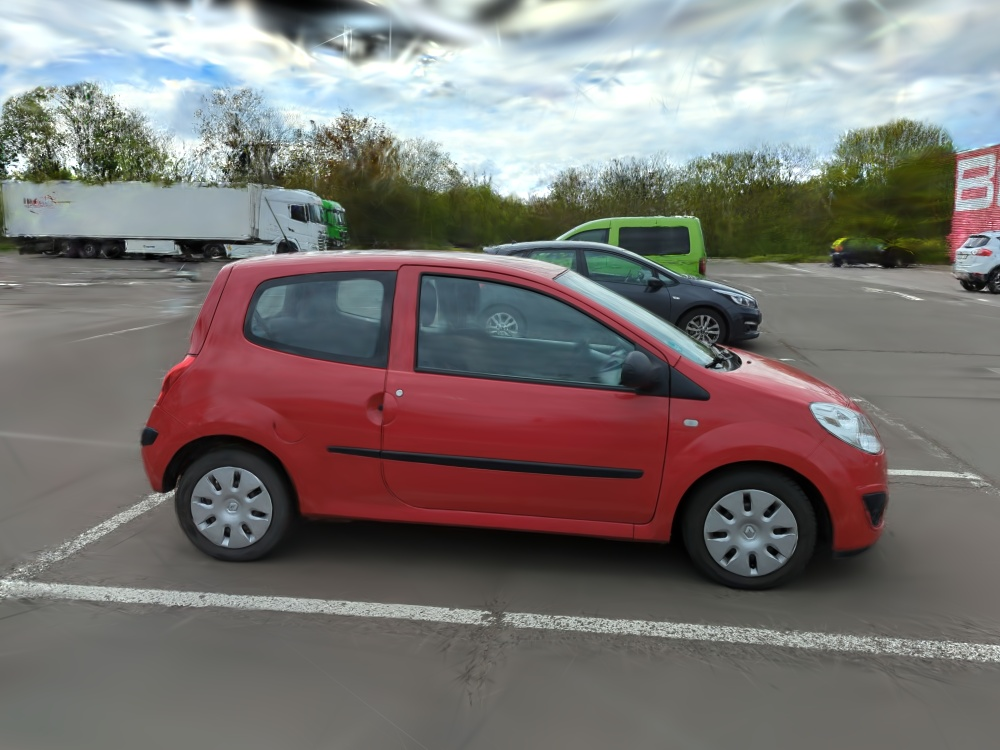
\includegraphics[width=\linewidth]{images/gaussiansplatting/stabgs/img-3.jpg}
    \caption{\textbf{Rendered view from GS scene.}}
    \label{fig:gs-view3-gs}
  \end{subfigure}
  \caption{\textbf{Gaussian Splatting based stabilization} Contrary to the homography-based solution, our trained GS is able to render the whole car.}
  \label{fig:gs-view3}
\end{figure}

The corresponding spin stabilized animation is proposed on Figure \ref{fig:gs-stabilized-gs-gif}. 

\begin{center}
  \animategraphics[autoplay,loop, poster=0,width=\linewidth]{5}{images/gaussiansplatting/stabgs/img-}{0}{35}
  \label{fig:gs-stabilized-gs-gif}
  \captionof{figure}{\textbf{Stabilized $360\degree$ spin path with GS} Whereas the car is not cropped anymore during stabilization, some details are missing on the car.}
\end{center}

The scene we considered is not prone to such undesired effect but it might occur during rendering that floaters artifacts appear. As we stabilize the camera path and render views at locations that were not originally observed, these artifacts are actually not very surprising. There floaters must be removed directly from the 3D scene itself, so that they are not render. We chose first, before delving into a floater removal algorithm, to slighly change minimal depth distance of the culling frutrum. Figures \ref{fig:gs-cullingfrustrum} and \ref{fig:gs-floaters} respectivelly present the core idea of such modification and its direct impact during rendering on an other scene (since the original one does not have such visible floaters). 


\begin{figure*}[htb!]
  \center
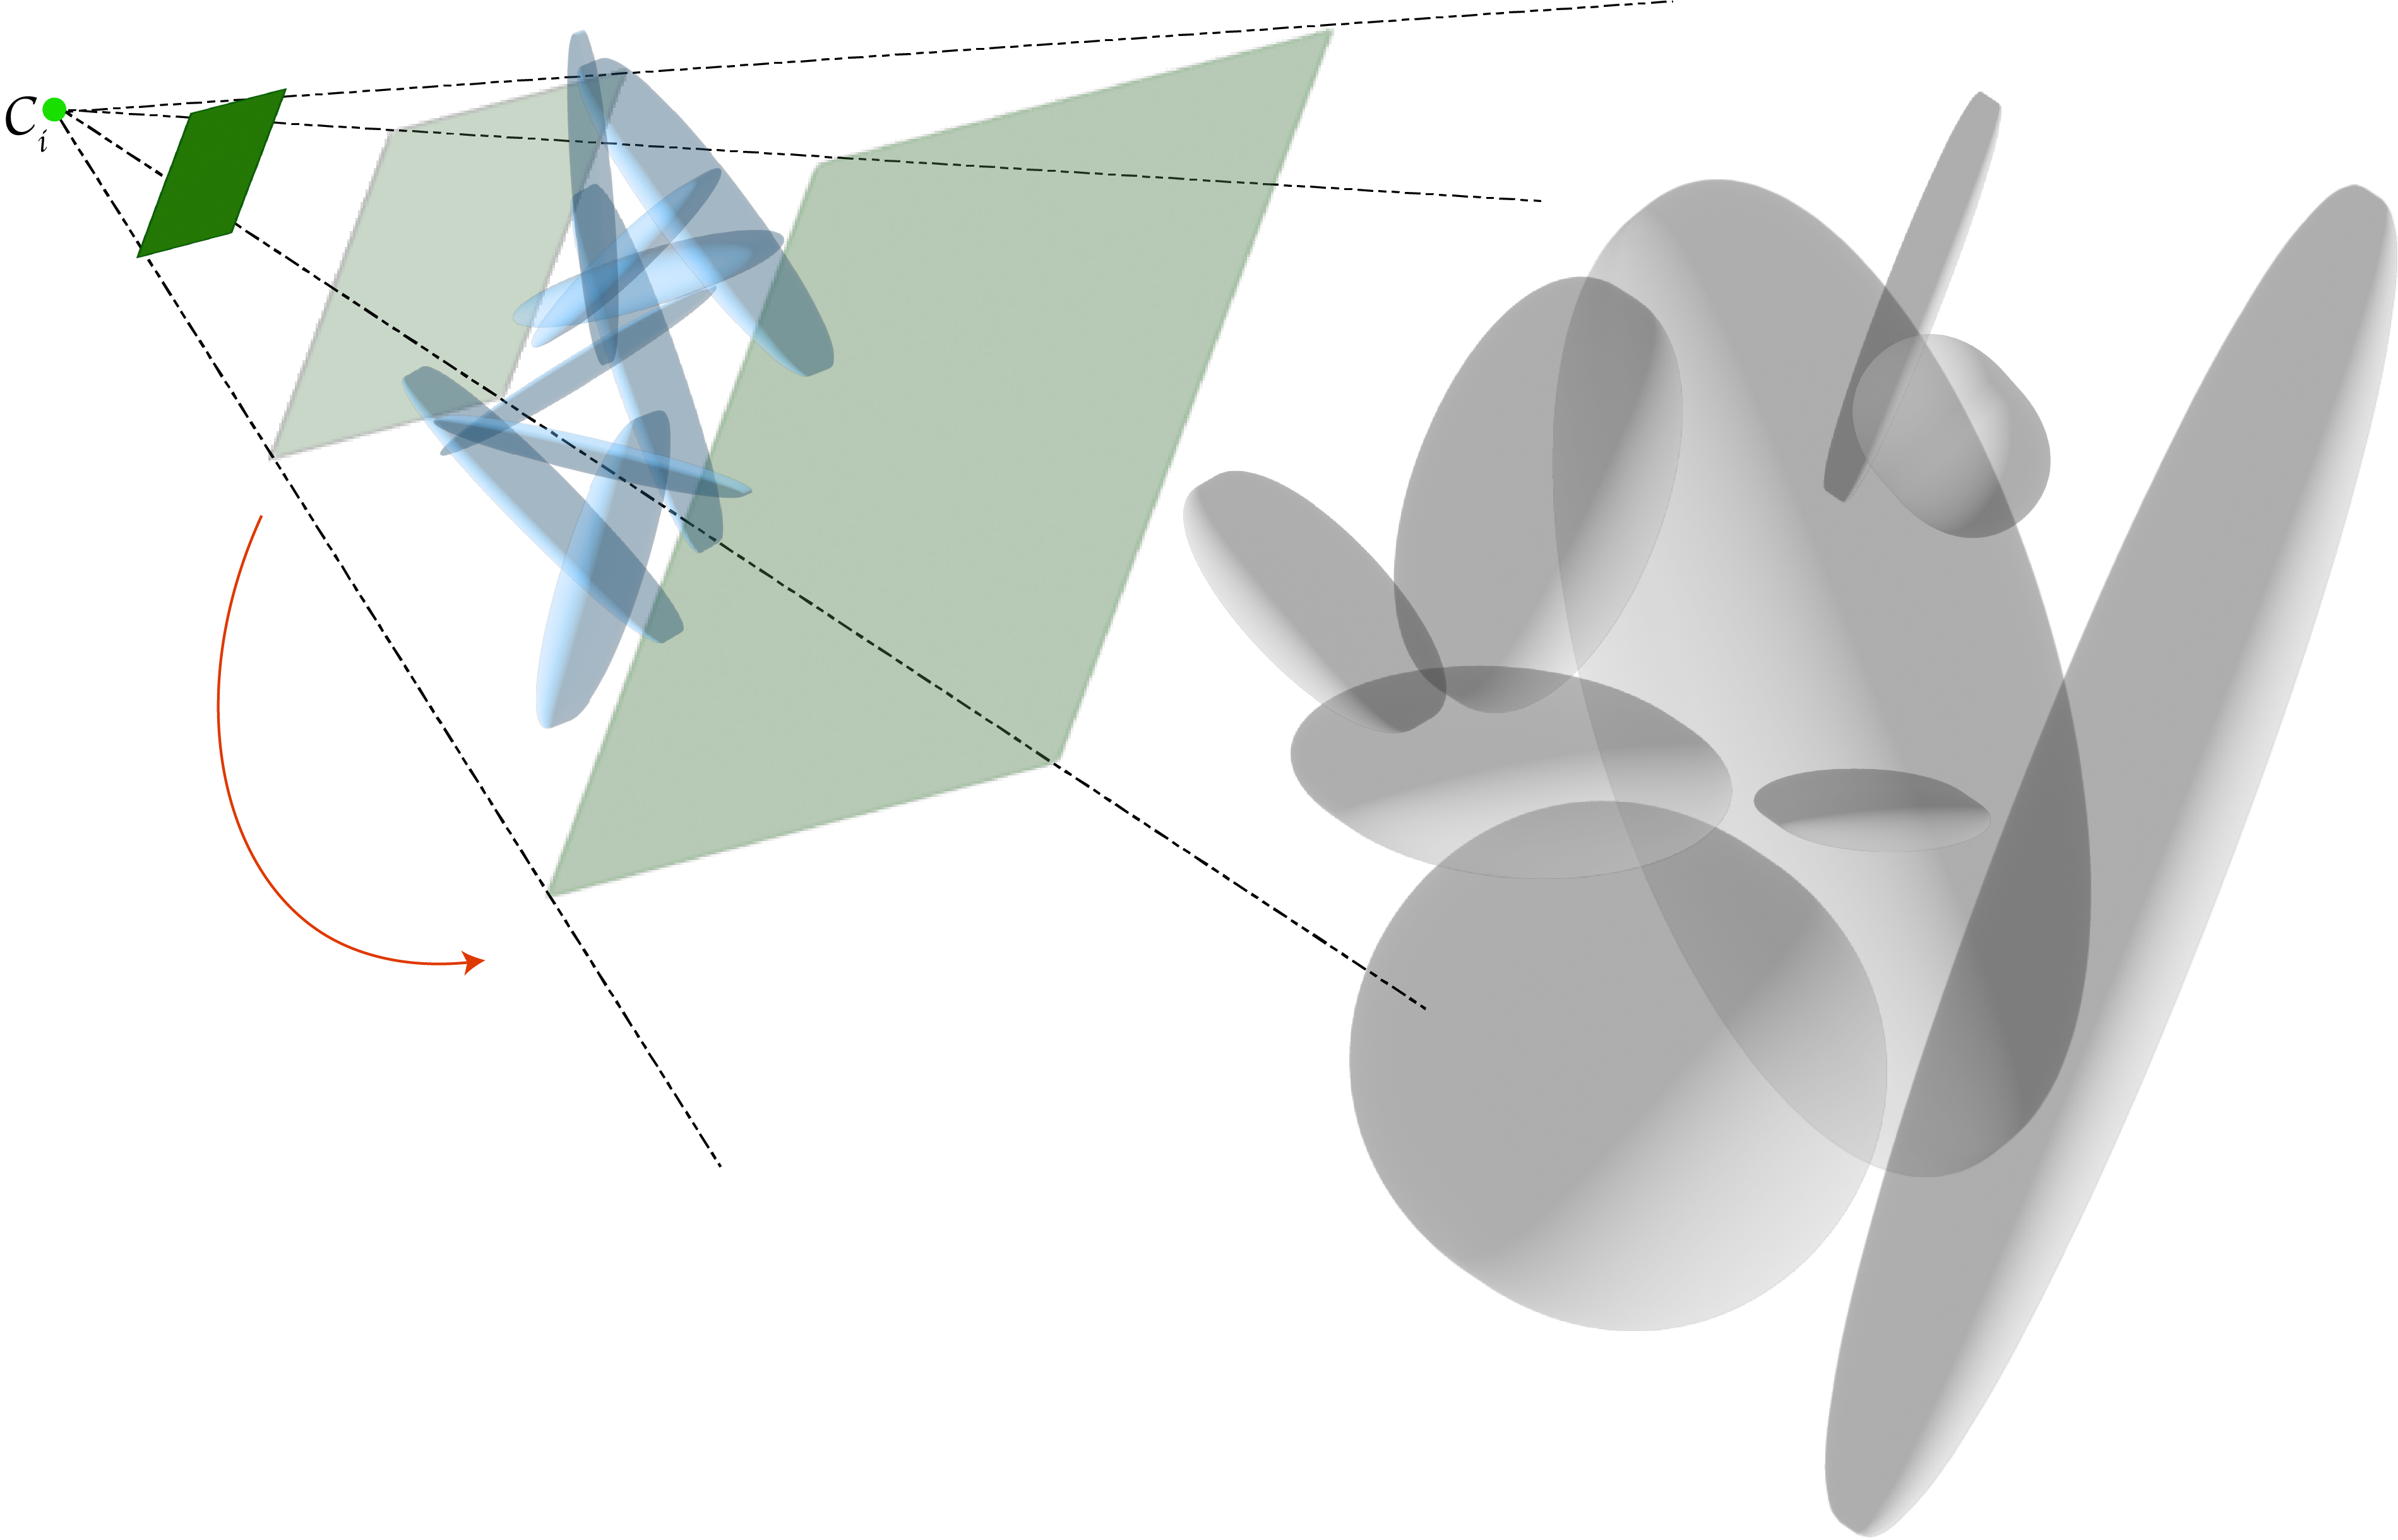
\includegraphics[width=.7\linewidth]{images/gaussiansplatting/gaussian-floaters.png}
\caption{\textbf{Floater artifacts visualization} Moving the minimal depth distance from which a gaussian fall into the culling frustrum enables to avoid rendering floaters. Such floaters are often non observable at training locations since they lie behind the camera.}
\label{fig:gs-cullingfrustrum}
\end{figure*}

The stabilization of the scene on Figure \ref{fig:gs-floaters} induced a small step back. Such a minor camera displacement has caused some floating gaussians to fall into the culling frustrum of this new position, and have thus been rendered. Restrict a bit the culling frustrum to avoid too closed gaussians to be rendered allow to easely get ride of them. 
 
\begin{figure*}[htb!]
  \center
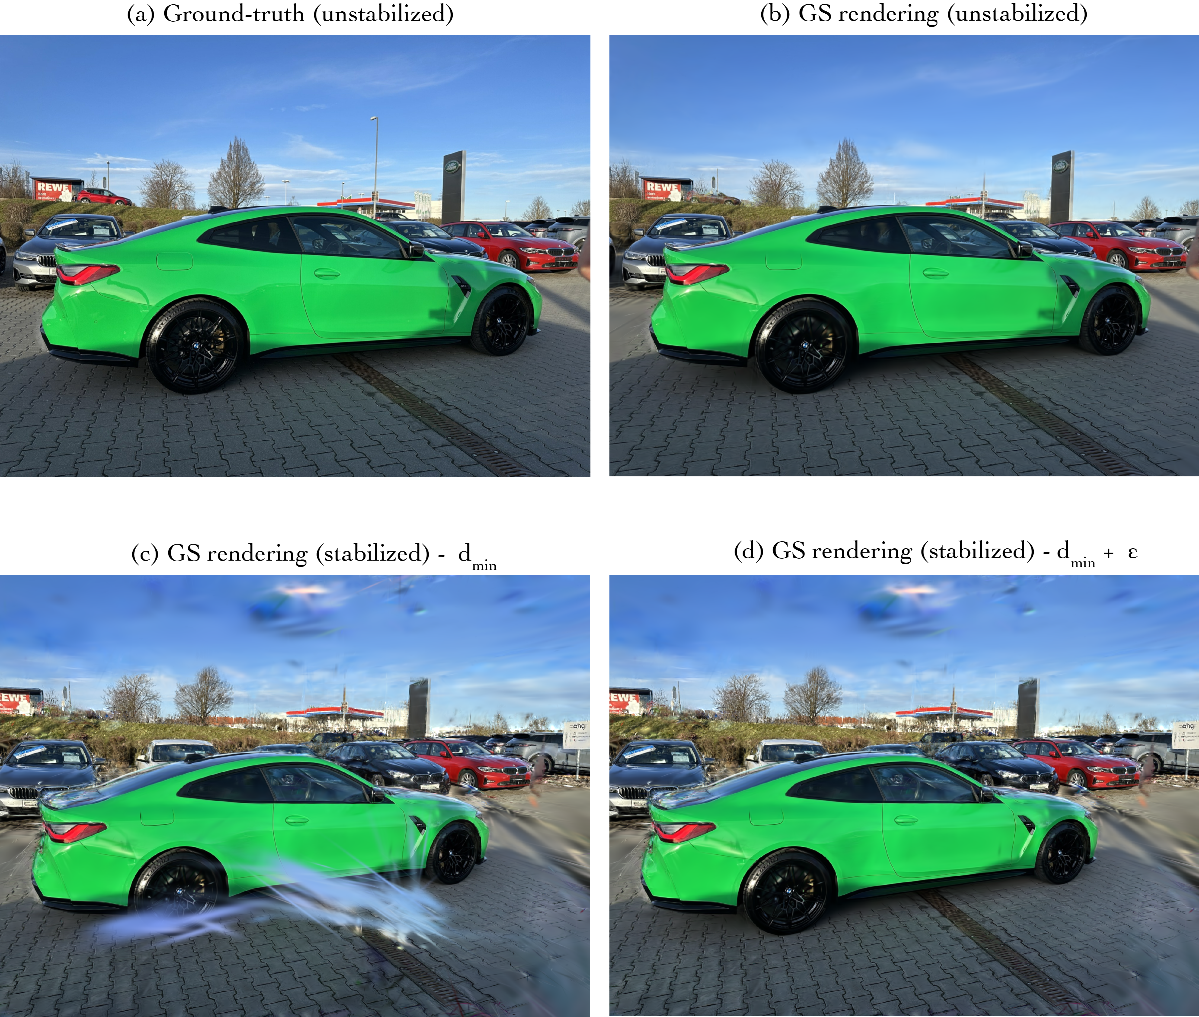
\includegraphics[width=.7\linewidth]{images/gaussiansplatting/gaussian-floaters-results.png}
\caption{\textbf{Floater artifacts rendering} Render the scene at training (unstabilized) locations does not induce any floater artifacts (see \textit{(b)}). However, once the scene is stabilized and the corresponding view rendered, small \textit{needle} artifact appear. Setting a higher minimal distance for a gaussian to fall into the culling frustrum allow to get ride of these floaters.}
\label{fig:gs-floaters}
\end{figure*}



\section{Experiments}
\ref{sec:gs-experiment}

\subsection{View-dependancy effect}

\subsection{Visual Hull}
We experiment in this section a novel way to get the initial point cloud $\mathcal{P}$ we need to start with for \ac{GS} training. As it has already been shown on Figure \ref{fig:gs-sfm} and explained in \ref{subsec:gs-sfm}, the point cloud COLMAP produces is extremely sparse: $\mathcal{P}$ has only roughly 4K points and most of them do not lie on the car surface. 

We consider a novel point cloud, termed $\mathcal{P}_{VH}$, that direclty leverages from a visual hull, a silhouette-from-motion based-concept. The main idea is rather straightforward, since it only requires to get the posed images and the corresponding binary masks. The Figure \ref{fig:gs-vh-concept} allows to grasp the visual hull concept. 

\begin{figure*}[htb!]
  \center
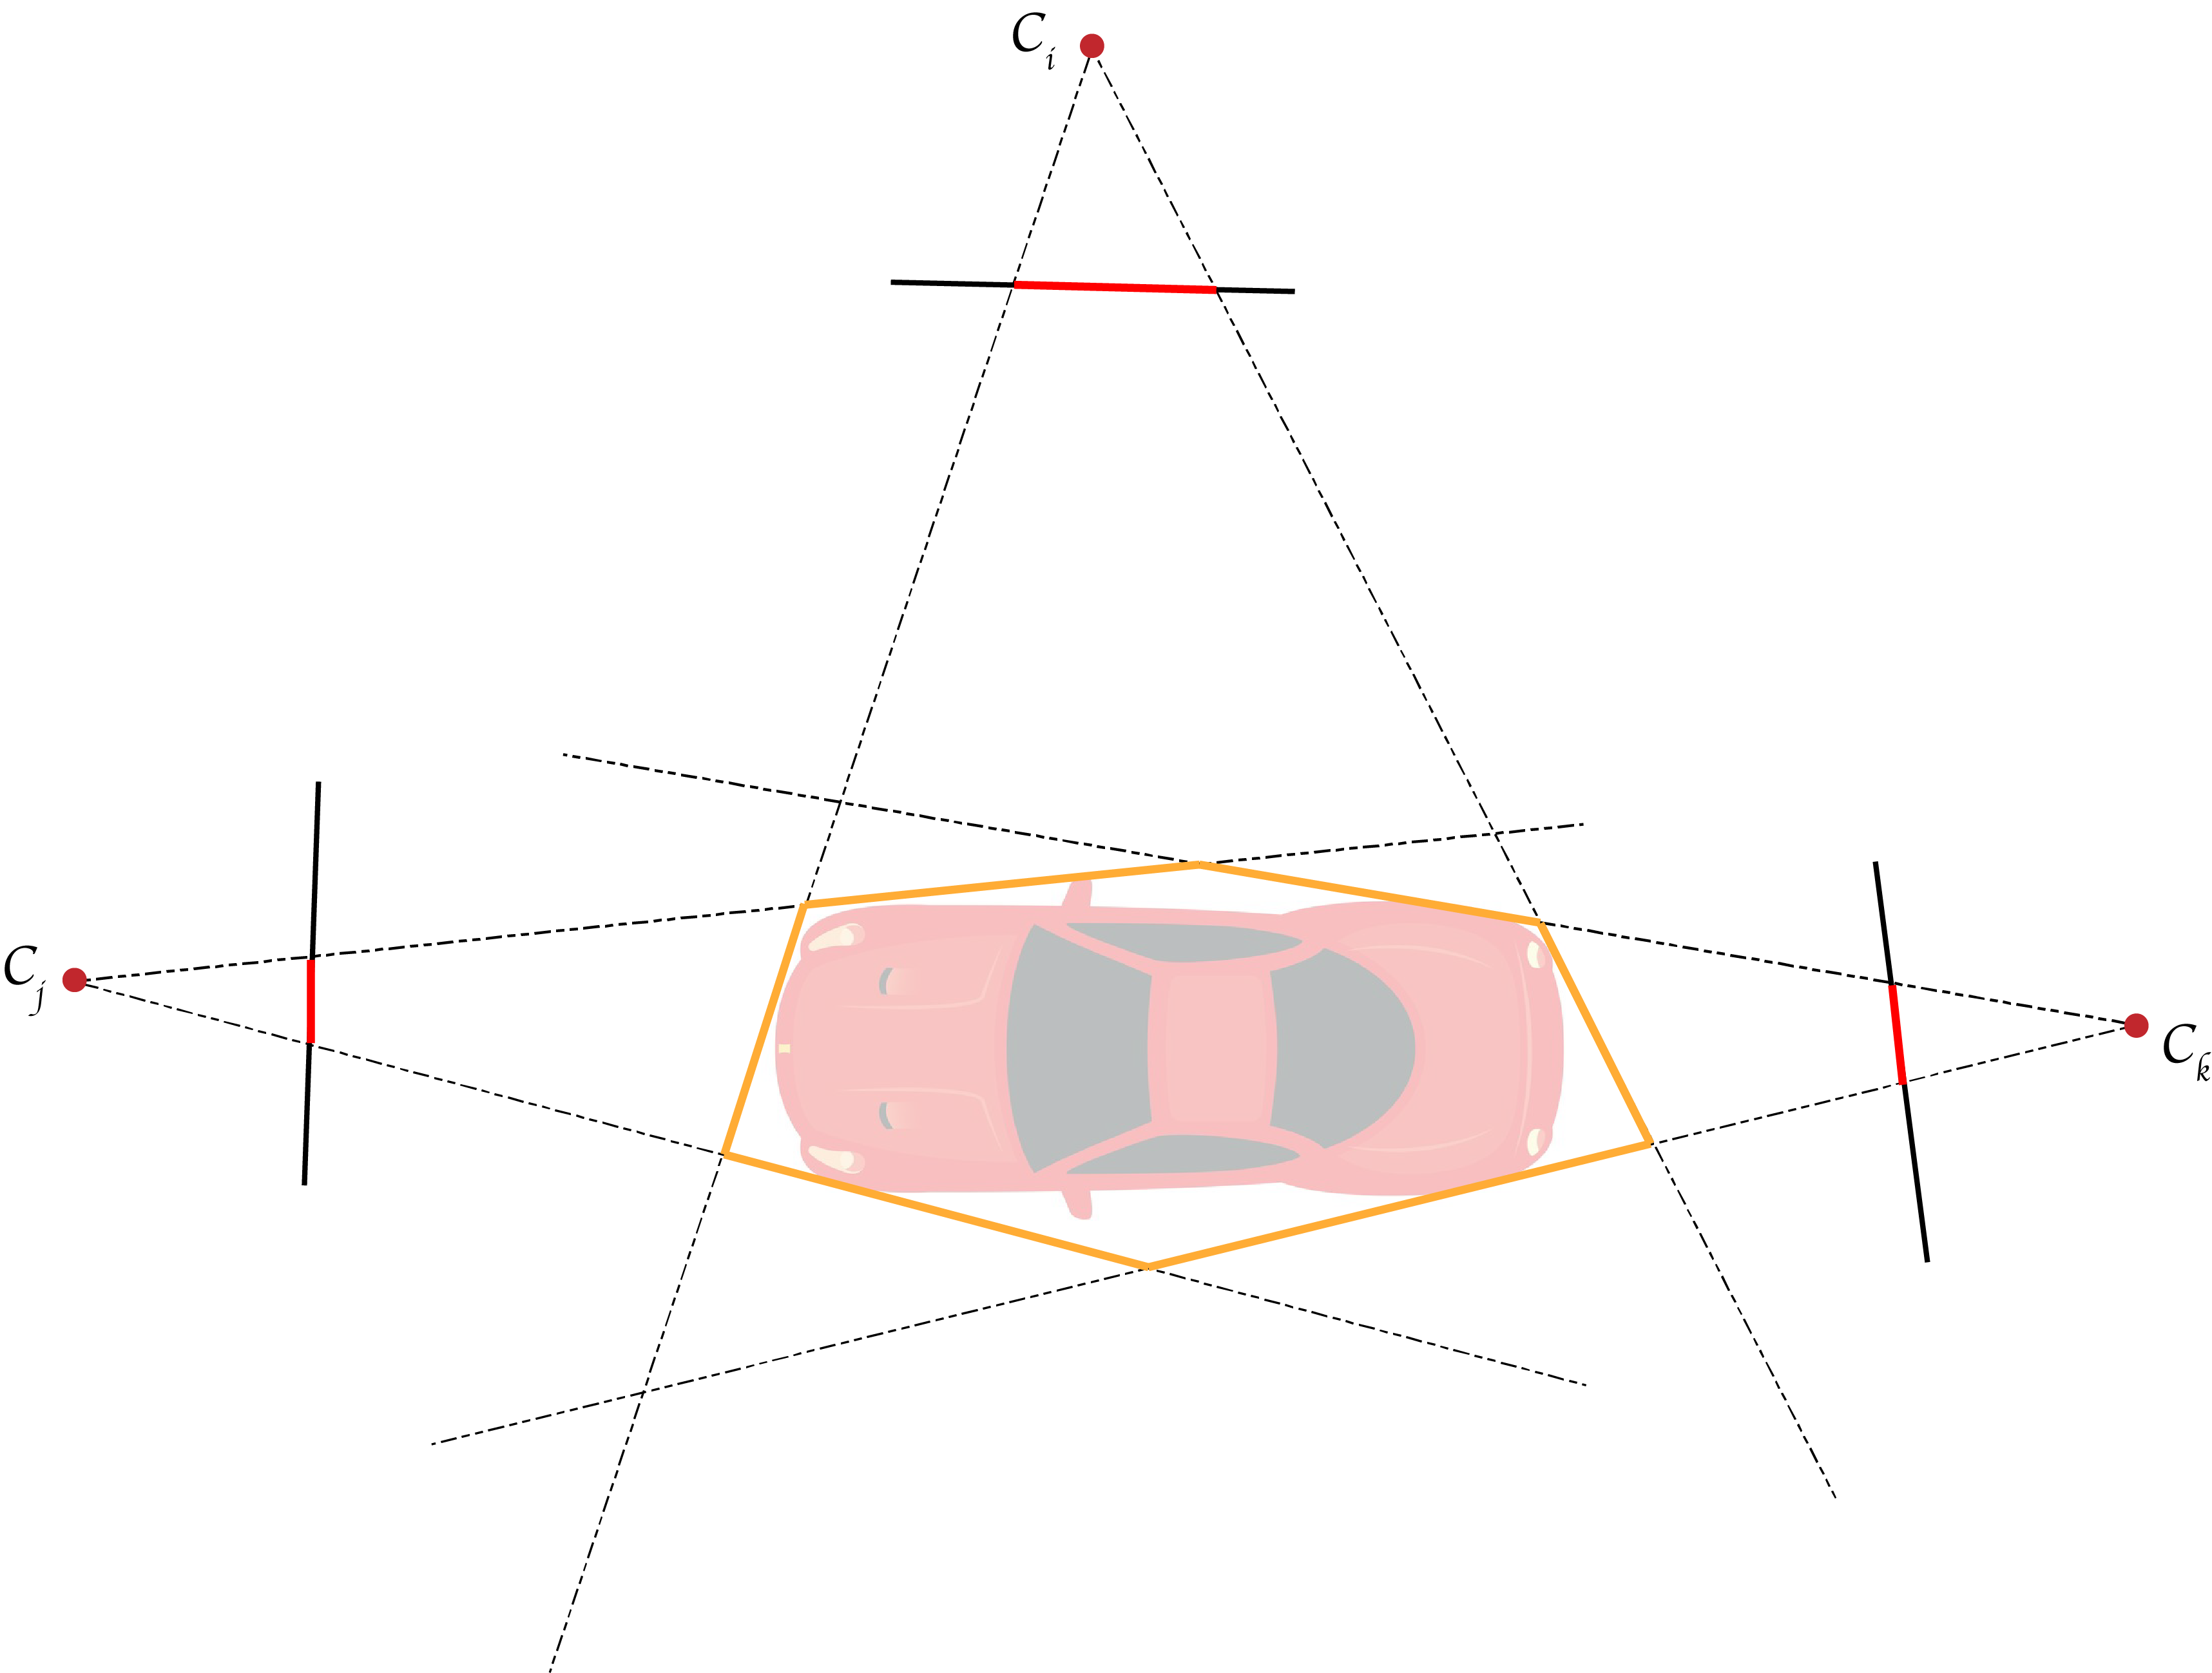
\includegraphics[width=.7\linewidth]{images/gaussiansplatting/visualhull-idea.png}
\caption{\textbf{Visual hull concept.} A visual hull is here built as the intersection of three 3D bounding cones from the silhouette masks. Such hull is almost convex in case of our car scenario. One can  sample 3D points within the visual hull to build a new dense point cloud.}
\label{fig:gs-vh-concept}
\end{figure*}

We present on Algorithm \ref{alg:gs-vh} the pseudo code that allow to generate such a visual hull and the corresponding dense coloured point cloud $\mathcal{P}_{VH}$ we can obtained on Figure \ref{fig:gs-vh-result}. 

\begin{algorithm}[h]
  \caption{Visual hull contruction}\label{alg:gs-vh}
  \SetKwInOut{Input}{input}
  \SetKwInOut{Output}{output}
  \SetKwInOut{Parameter}{parameter}
  \Input{Images $\mathcal{I}$, Silhouette mask $\mathcal{S}$}
  \Parameter{Intrinsic and extrinsic camera parameters $\pi=K[R|t]$}
  \Output{Visual hull-based point cloud $\mathcal{P}_{VH}$ } 
  \medskip
  \KwResult{$\mathcal{P}_{VH}$ can be densely sampled}
  \medskip
  $bbox \gets \mathbf{build3DBB}()$ \tcp*[l]{Create a vanilla 3D bounding boxe}
  $P_{3D} \gets \mathbf{sampleDensely}(bbox)$\hspace{.4cm}\textcolor{gray!80}{\# 
    [$N_{pts}$,3]} \tcp*[l]{Sample points in the BB}

   $P_{2D} \gets \mathbf{project}(P_{3D},\pi)$ \hspace{.4cm}\textcolor{gray!80}{\# 
    [$N_{pts}$,2]} \tcp*[l]{Reproject on image plane }
    
    $idx_{valid} \gets \mathbf{keepValidPoints}(P_{2D},\mathcal{M})$ \hspace{.4cm}\textcolor{gray!80}{\# 
    [$N_{pts}$,1]} \tcp*[l]{Boolean. 1 if valid, 0 otherwise}

    $P_{3D}^{(refined)} \gets P_{3D}[idx_{valid}]$ 

    $P_{VH} \gets \mathbf{setRGBcolor}(P_{3D}^{(refined)},P_{2D},idx_{valid},\mathcal{I})$ \tcp*[l]{Set RGB color to the point cloud through bilinear interpolation}
\end{algorithm}


\begin{figure*}[htb!]
  \center
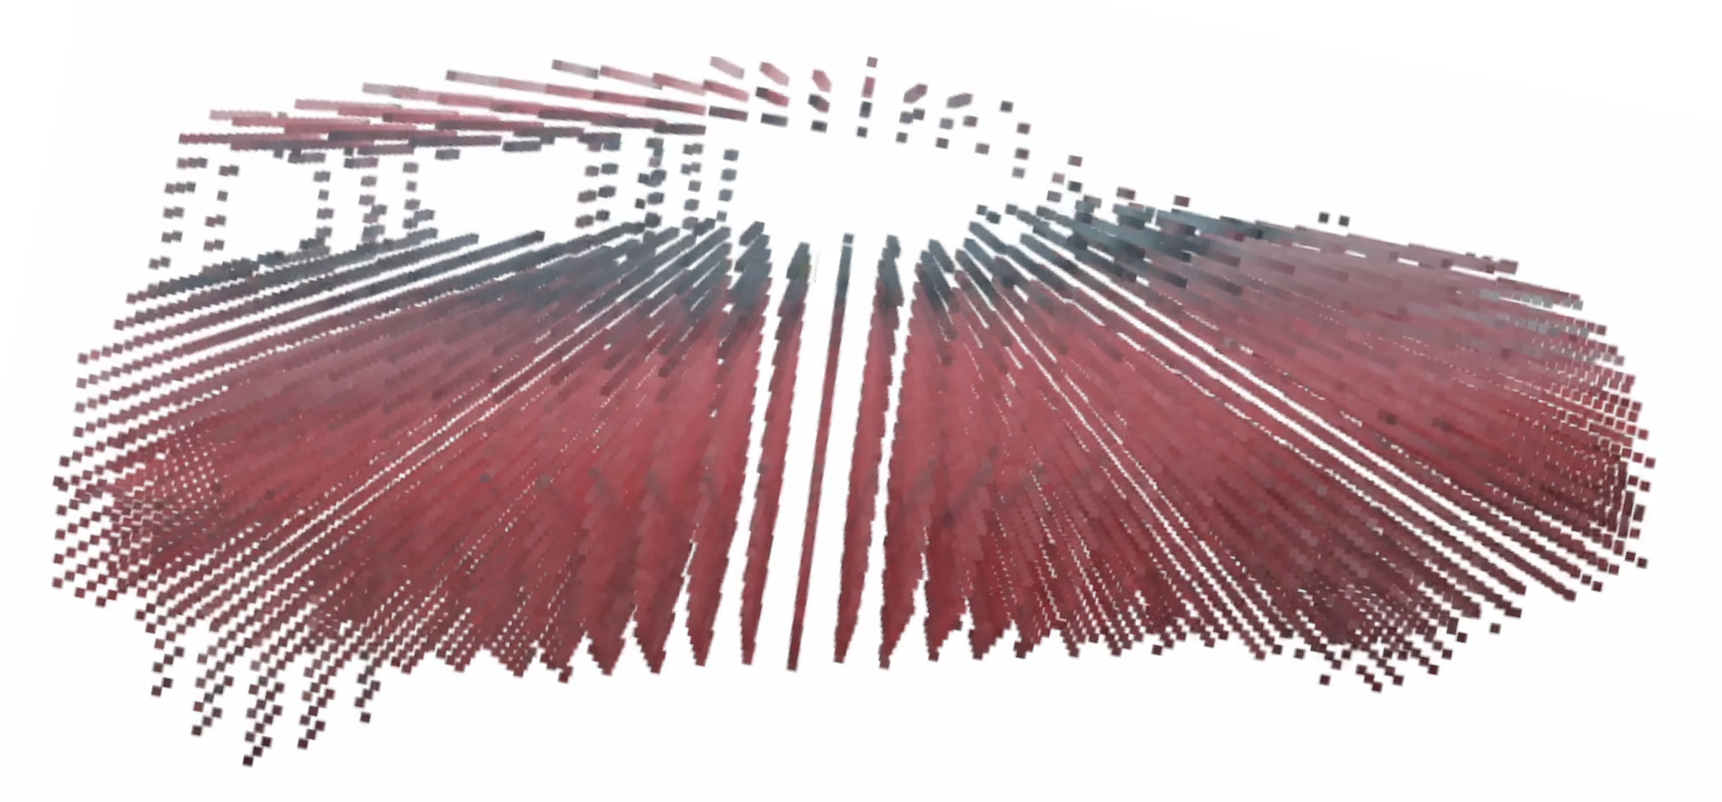
\includegraphics[width=.7\linewidth]{images/gaussiansplatting/visualhull-res.png}
\caption{\textbf{Visual hull concept.} A visual hull is here built as the intersection of three 3D bounding cones from the silhouette masks. Such hull is almost convex in case of our car scenario. One can  sample 3D points within the visual hull to build a new dense point cloud.}
\label{fig:gs-vh-result}
\end{figure*}

However, the visual hull-based point cloud also remains incomplete in its current form since it leaves a large number of areas without any points in the 3D scene: sky, ground or surrounding cars are not represented by any gaussians when the \ac{GS} training starts. Even though the optimization process move some of these gaussians toward these under-reconstructed areas, the final point cloud is too sparsely densified outside of the car itself. It might not be an issue as soon as we extensively want to reconstruct and synthesize novel views of the car. Since we performing neural rendering on an explicit gaussian point-clouds, undesired gaussians (such as these needle floaters artifact described on Figure \ref{fig:gs-floaters}) might be rasterized \textit{over} the car.  

One naive yet effective solution is thus to merge the two original point cloud we have at our disposal: $\mathcal{P} = \mathcal{P}_{COLMAP} \cup \mathcal{P}_{VH}$. We therefore expect to benefit from the higher point density of $\mathcal{P}_{VH}$ on the car and from the better background representation of $\mathcal{P}_{COLMAP}$ too. Whereas it increases the original volume of gaussians to optimize, and thus the training time, rendering at stabilized locations are more visually pleasant, with better car inner details synthesis. The figure \ref{fig:gs-vishull-comp} and Table \ref{table:gs-vh-influence} both visually and quantitatively confirm the benefit of this point cloud merging strategy. 

\begin{figure*}[htb!]
  \center
\includegraphics[width=.9\linewidth]{images/gaussiansplatting/vishull-comp.png}
\caption{\textbf{Point cloud initilization influence.} COLMAP-based point \textit{(left)} cloud yields a satisfying result, even though some inner details are missed. The visual hull based \textit{(center)} initialization method produce sharper results in the car, but floaters are rendered on the roof the car. Merging the two point cloud \textit{(right)} allows to get the best of both configuration.}
\label{fig:gs-vishull-comp}
\end{figure*}


\begin{table}[htp!]
  \caption{\textbf{VisualHull influence} Quantitative results how influenciable the original point cloud can be on the GS rendering performance.}
  \label{table:gs-vh-influence}
  \centering%\begin{center}
  \begin{adjustbox}{width=\linewidth}
  \begin{tabular}[h]{c||ccccccc}
  \hline
   PC initialization & \multicolumn{3}{c}{Full Image} & \multicolumn{3}{c}{Car only} \\
   &  SSIM ($\uparrow$) & PSNR ($\uparrow$) & LPIPS ($\downarrow$) & SSIM ($\uparrow$) & PSNR ($\uparrow$)) & LPIPS ($\downarrow$)\\
  \hline
  COLMAP-SfM  & 0.787  & 28.592 & 0.334 & 0.990 & 41.998 & 0.020 \\
  VisualHull & 0.736 & 26.850 & 0.392 & 0.990 & 41.835  & 0.018 \\
  COLMAP-SfM + VisualHull & \cellcolor{red!25}0.810 & \cellcolor{red!25}29.288 & \cellcolor{red!25}0.314 & \cellcolor{red!25}0.993 & \cellcolor{red!25}43.452  & \cellcolor{red!25}0.014 \\
  \hline 
  \end{tabular}
  \end{adjustbox}
  %\end{center}
  \end{table}

\subsection{Revisiting the ADC strategy}

As \citep{zhang2024pixel}

\section{Conclusion}
